% README screenshot of paper Fig. 1 - layout copied from the paper source,
% caption shortened and stripped of cross-references.
\documentclass[border=8pt]{standalone}
\usepackage{newtxtext,newtxmath}
\usepackage{graphicx}
\usepackage{booktabs}
\graphicspath{{../../../}}
\begin{document}
\begin{minipage}{16.5cm}
\small
\centering
\begin{tabular}{@{\hskip 0.06in}c@{\hskip 0.06in}c@{\hskip 0.06in}c@{\hskip 0.05in}c}
   AR & MQAR & MQAR & \\
   (a) Linear Model & (b) Linear Model & (c) Full Model & \\
  \cmidrule(lr){1-3}
    \raisebox{-0.5\height}{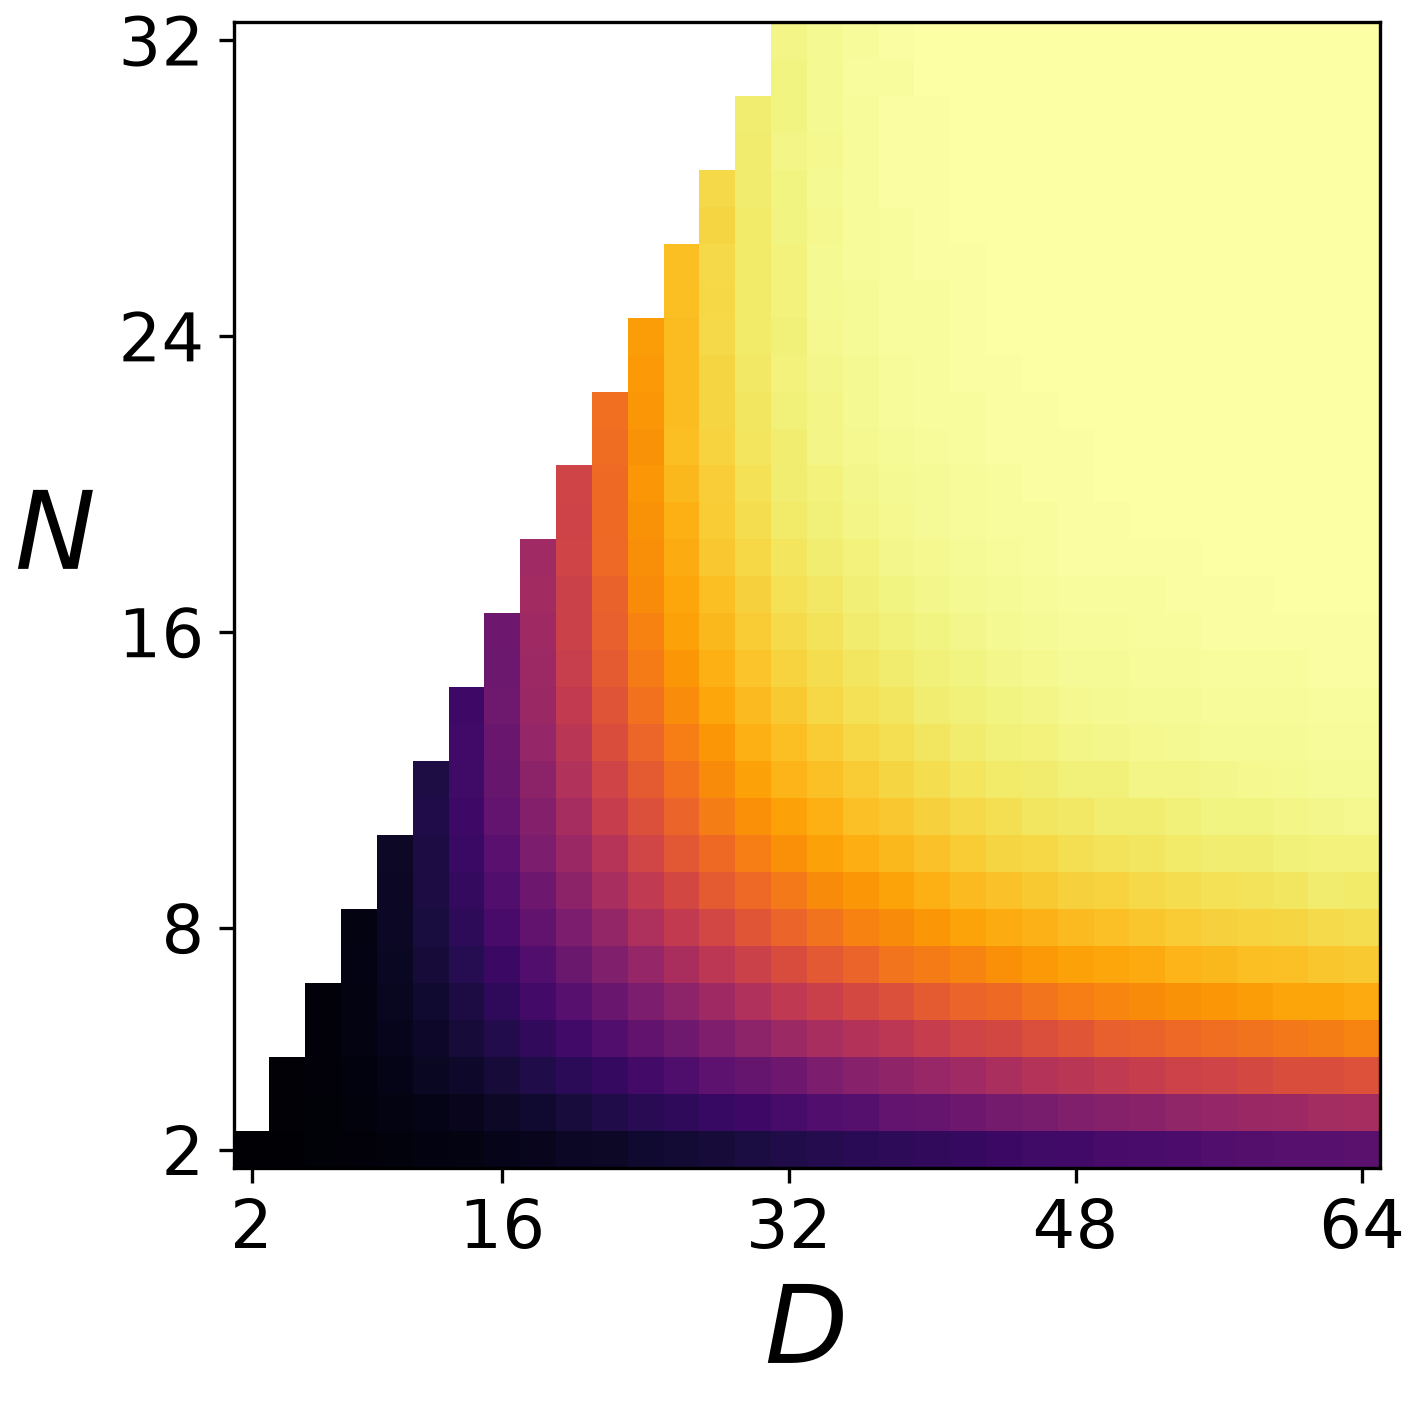
\includegraphics[width=0.31\linewidth]{figures/appendix/AR__D_N__linear_trained__regime_2.png}} &
    \raisebox{-0.5\height}{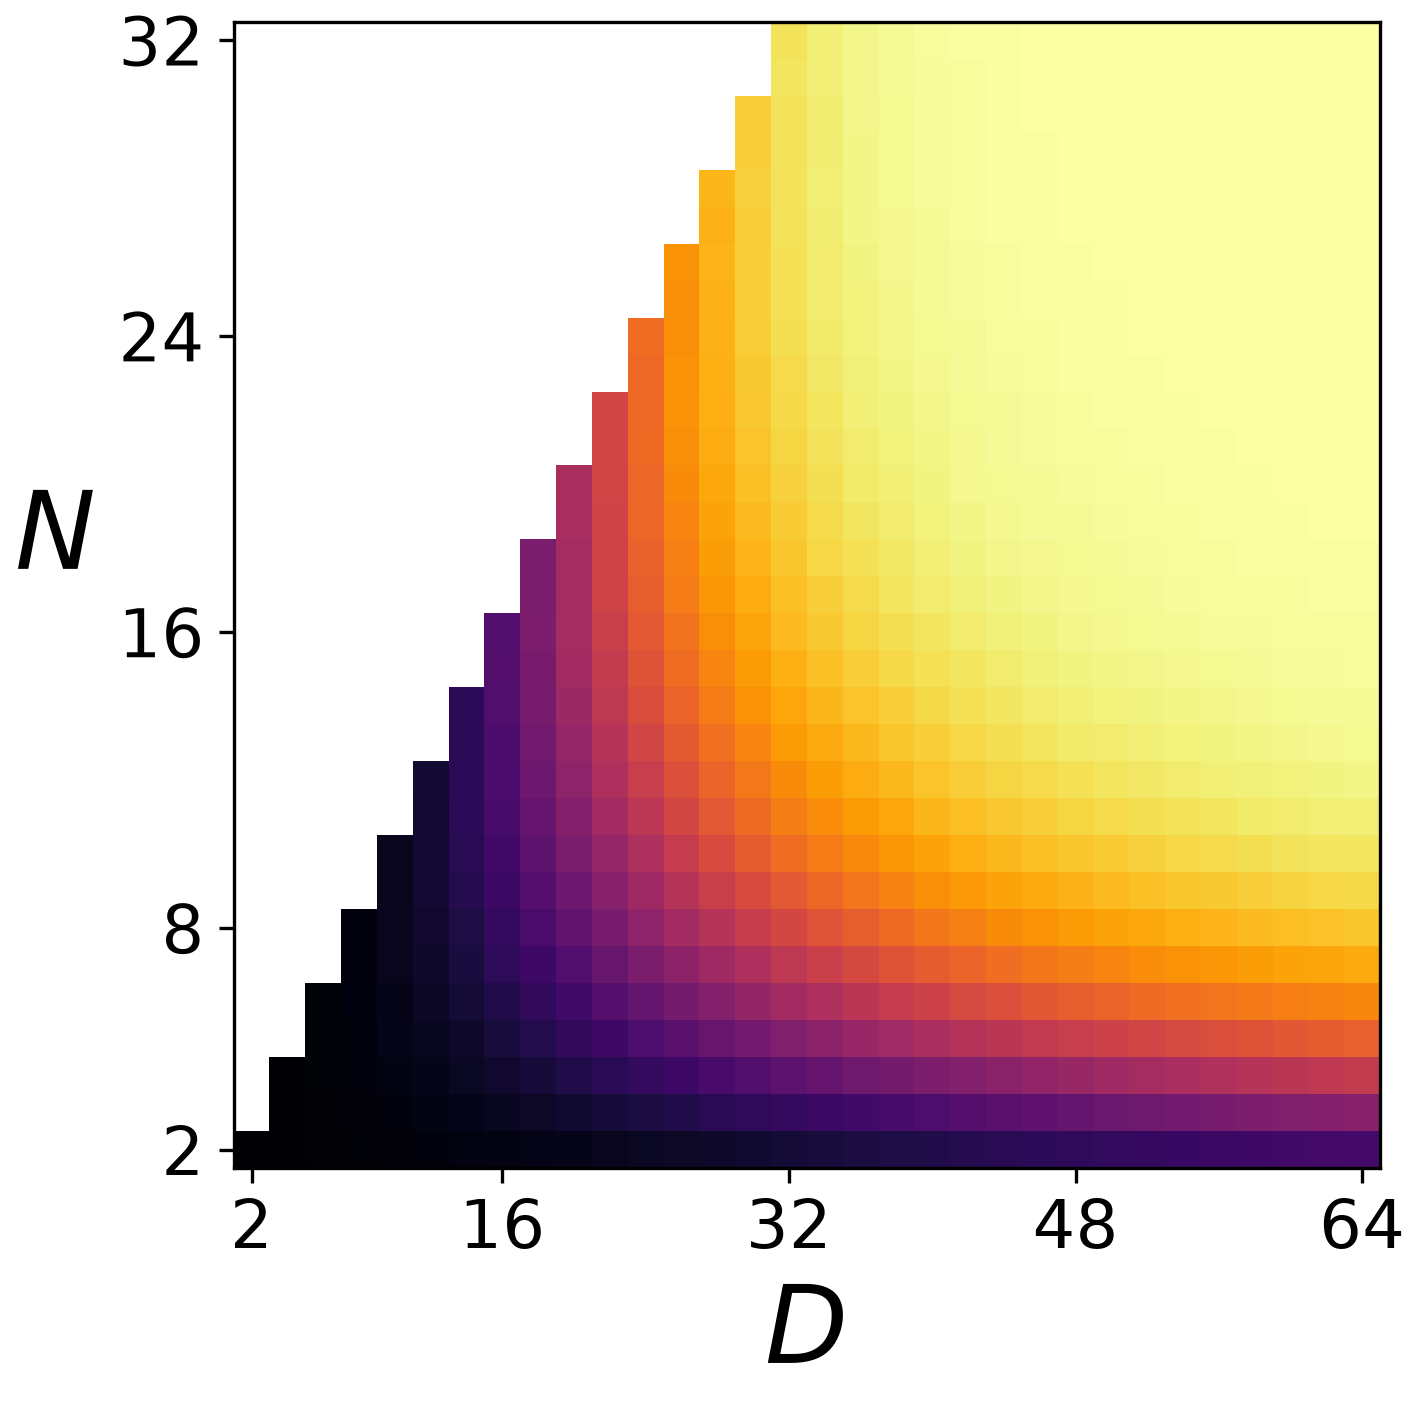
\includegraphics[width=0.31\linewidth]{figures/MQAR__D_N__linear_trained__regime_2.png}} &
    \raisebox{-0.5\height}{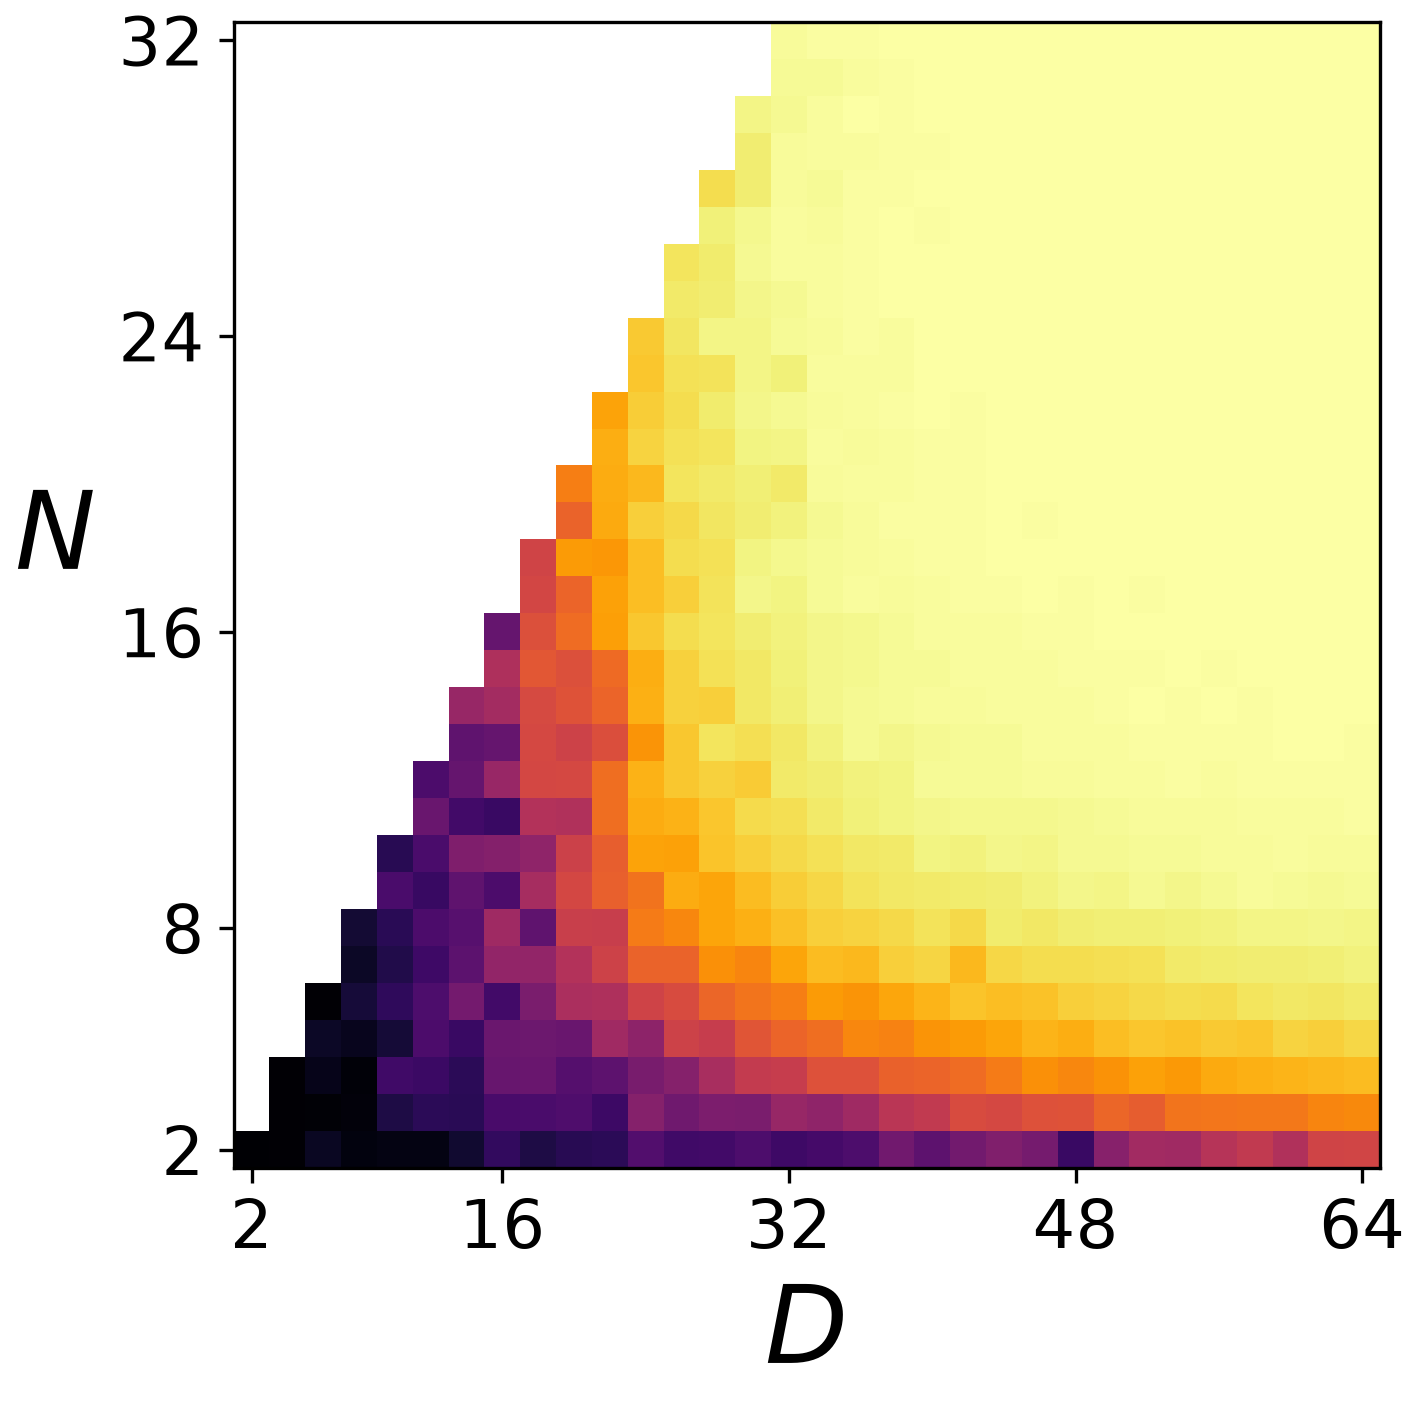
\includegraphics[width=0.31\linewidth]{figures/MQAR__D_N__full_trained__regime_2.png}} &
    \raisebox{-0.5\height}{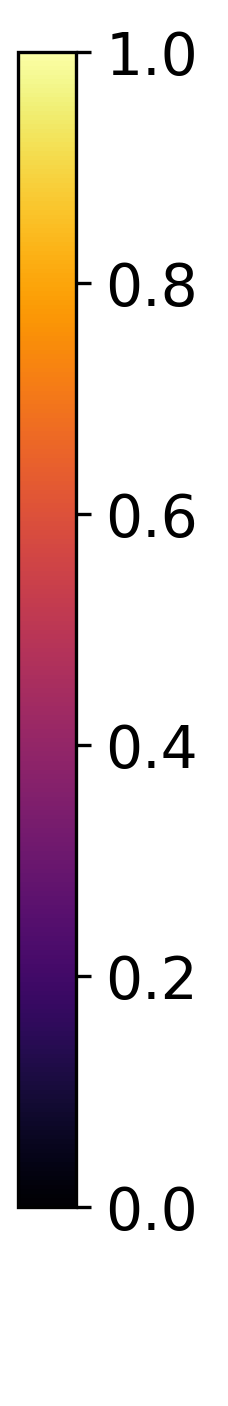
\includegraphics[width=0.045\linewidth]{colorbar.png}}
 \\
    \raisebox{-0.5\height}{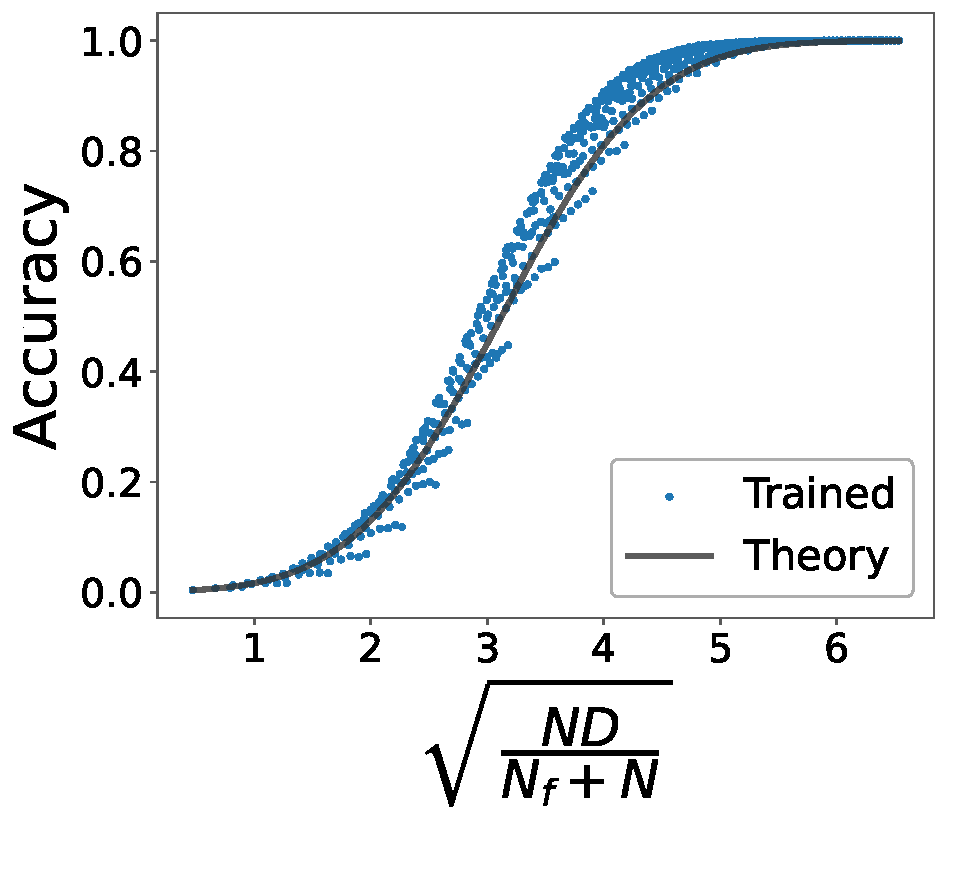
\includegraphics[width=0.31\linewidth]{figures/AR__D_N__linear_trained__regime_2__acc_curve__sigma_inv__main.pdf}} &
    \raisebox{-0.5\height}{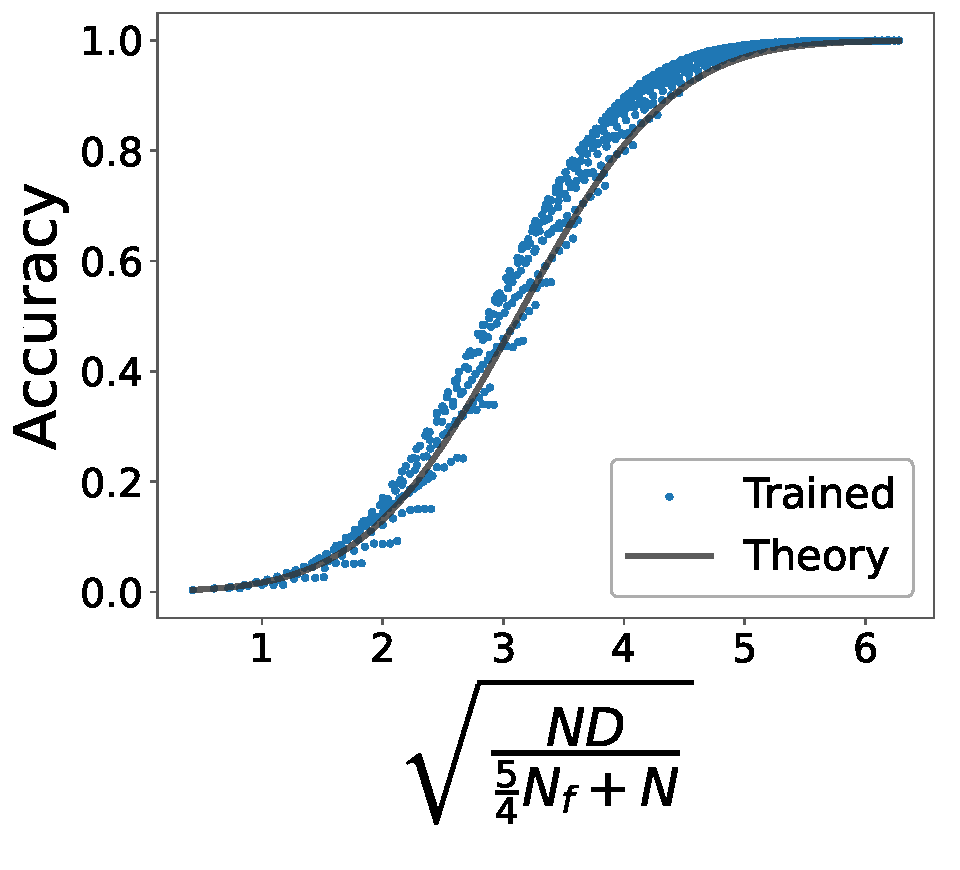
\includegraphics[width=0.31\linewidth]{figures/MQAR__D_N__linear_trained__regime_2__acc_curve__sigma_inv__main.pdf}} &
    \raisebox{-0.5\height}{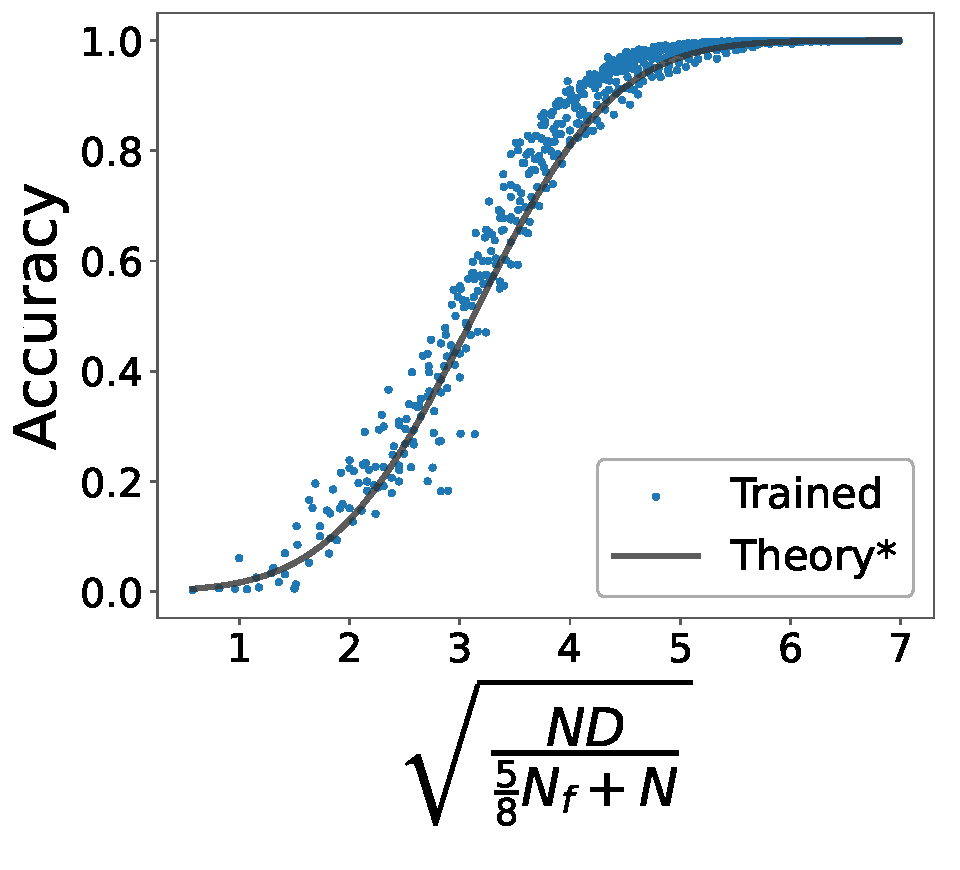
\includegraphics[width=0.31\linewidth]{figures/MQAR__D_N__full_trained__regime_2__acc_curve__sigma_inv__main.pdf}} &
 \\
 \end{tabular}
\end{minipage}
\end{document}
